\documentclass[sigconf]{acmart}

\usepackage{hyperref}

%\usepackage{endfloat}
%\renewcommand{\efloatseparator}{\mbox{}} % no new page between figures

\usepackage{booktabs} % For formal tables

\settopmatter{printacmref=false} % Removes citation information below abstract
\renewcommand\footnotetextcopyrightpermission[1]{} % removes footnote with conference information in first column
\pagestyle{plain} % removes running headers


\graphicspath{{images/}}


\begin{document}
\title{Big Data and the Issue of Privacy}


\author{Ashley Miller}
\orcid{HID329}
\affiliation{%
  \institution{Indiana University}
  \date{November 2017}
}
\email{admille@iu.edu}



% The default list of authors is too long for headers}
\renewcommand{\shortauthors}{G. v. Laszewski}


\begin{abstract}
The collection, analysis, and dissemination of findings from big data can provide benefits to society across a variety of industries including health care, education, law enforcement, and commercial retailers, to name a few. However, with benefits, also comes caveats, risks, and even significant harm when this process of harnessing big data does not go as planned. One prominent discussion point around the use of big data is around privacy. In today's age of sharing information, can one really expect privacy given all the methods in which they can share information? What impact can data breaches have on a person's (or company's) personal information, security, and livelihood? While there are techniques and tools that have been implemented to help minimize the risk, is a data breach more a matter of \textit{if} it occurs or more so \textit{when} occurs? We will seek to address these questions as we explore how the increasing and ever changing space of online behavior, data mining, and big data analytics affects today's experience with maintaining privacy.  
\end{abstract}

\keywords{i523, hid329, big data, privacy, security, data mining}

\maketitle

\section{Introduction}

As defined by Merriam-Webster, privacy is the ``quality or state of being apart from company or observation" \cite{Merriam-Webster2017}. As we explore the world of internet behavior and big data, the question is: should we ever expect \textit{privacy} as we are constantly being observed in this space? The Supreme Court has weighed in on this debate by stating that ``one cannot have a reasonable expectation of privacy in information that is given to third parties or made accessible to the public" \cite{Review2014}. However, the government sector itself is one of the biggest data collectors across various agencies and hundreds, if not, thousands of databases \cite{Review2014}. With the vast amount of data collected by these agencies, ranging from political contributions to payroll, the definition of personal identifiable information (PII) can vary even across state lines as well as the laws and policies that govern them \cite{Agelidis2016}. 

\section{What is Personal Identifiable Information? (PII)}

Despite the differences that may exist in what constitutes PII and what does not, there are main components these definitions have in common. PII is defined as an individual's name (first name and last name initial or the full last name) in conjunction with one of the following \cite{Agelidis2016}:

\begin{itemize}
  \item An individual's social security number 
  \item A state identification or driver's license number
  \item Information related to an individual's protected health information, which could include health status or payment method
  \item A password to access an account such as a debit or credit card
\end{itemize} 

While the Federal Trade Commission (FTC) provides guidelines and regulations in regards to storing personal information, they do not necessarily have an explicit definition for what constitutes PII \cite{Agelidis2016}. Due to this, ``reputation-implicating information" is not included \cite{Agelidis2016}. However, this does not mean that companies are absent from blame when data breaches occur that inflict reputational harm. Fair information practices (FIPs) help to give guidance to organizations as they seek to balance the responsibility of collecting and maintaining personal information but also adhere to data security and privacy laws \cite{Culnan2009}. Despite this, the United States has no one law or set of laws that would require all organizations to follow FIPs as separate laws cover particular industries such as the Health Insurance Portability and Accountability Act (HIPAA) for health care organizations, Fair Credit Reporting Act (FCRA) for consumer credit agencies, as well as many others \cite{Culnan2009}. These separate set of provisions along with inconsistent, and even outdated, laws and practices from state to state, call into question further how one's privacy can be compromised.

\section{How Can Privacy Be Compromised?}

Cunan and Williams outline two key privacy issues in Figure~\ref{f:PrivacyIssues} regarding information reuse and unauthorized access \cite{Culnan2009}. 

\begin{figure}[!htb]
  \centering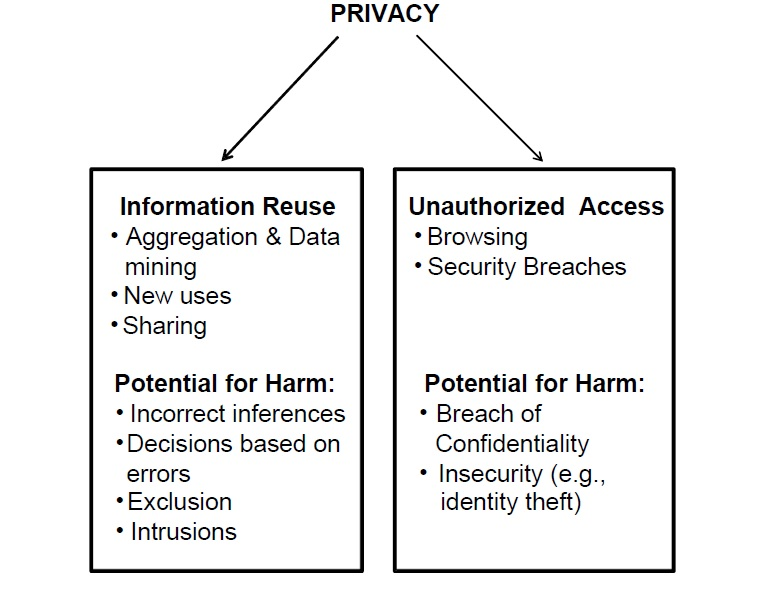
\includegraphics[width=\columnwidth]{images/privacy.jpg}
  \caption{Privacy Issues}\label{f:PrivacyIssues}
\end{figure}

Data breaches would fall into the category of \textit{unauthorized access}. As of information presented in 2009, it was then estimated that nearly 250 million records had been exposed to some sort of data breach \cite{Cavoukian2012}. Given recent news of data breaches among major companies such as Yahoo!, Target, and Experian, recent figures now estimate that number to be 825 million records \cite{Shell2017}. Data breaches can be described as a means to extort, expose or embarrass others \cite{Agelidis2016}. Among a sample of 500 investigations, it was estimated that nearly nine of out ten data breaches could have been prevented \cite{Culnan2009}. 

Another way privacy can be compromised is when previously collected data is reused for a purpose in which it was not originally intended. A common data mining example cited is when Target used consumer purchasing information to predict pregnancy among consumers \cite{Xu2014}. When coupons for baby and pregnancy related products were sent to a teenager's house, a local Target store received complaints from an irate father who only later found out that his teenage daughter was, in fact, pregnant \cite{Xu2014}. While data mining and predictive analytics can provide benefits to consumers and companies, this one example brings up an interesting debate as to where the privacy line should be drawn when data is used for other purposes that a consumer may not be fully aware of or understand.

\section{Where Can Privacy Be Compromised?}

Like local retail stores such as Target or even online providers such as Amazon, consumers provide their data across a variety of industries, situations, platforms, and methods. Areas where PII could be compromised include but not are limited to:

  \subsection{Mobile} 

Smart phone applications alone can house a wealth of data among individual users \cite{Tene2013}. In addition, sensors such as microphones, cameras, and global positioning systems (GPS) can offer more information as to what a user sounds like, looks like, and even their travel patterns \cite{Tene2013}. It's hard to say whether consumers are fully aware of these possible data collection methods and what measures, if any, they take to protect their privacy on a mobile device such as turning off location finding features or password protecting accounts. However, a study conducted by Dimensional Research shows that one out of every five security professionals surveyed have had their company experience a data breach from their mobile device while nearly one out of four state they are unsure if one has occurred \cite{Collett2017}. 

  \subsection{Health Care} 

A patient's family history, prescriptions taken, diseases, and disorders are stored by physicians' offices and can live in electronic medical records (EMR) across the globe. Health insurance companies are also another player in collecting and maintaining big data on their consumers. While harnessing this information can provide substantial benefit to developing outcomes and even identifying trends, it can also be at risk of being compromised if not properly secured and maintained \cite{Tene2013}. One such example includes nearly 80 million records that were compromised from Anthem in 2015 \cite{Akpan2016}. Considering these records can contain home addresses, social security numbers, and even names of partners and children, the damage one can inflict to an individual can be extensive and overall, the impact of these data breaches are said to have cost the health care industry nearly 5.6 billion dollars per year \cite{Akpan2016}.

  \subsection{Education} 

Even in the realm of education, individual information around academic performance, class behavior, as well as intellectual disabilities can be at risk of being compromised \cite{Bathon2013}. Higher education systems in particular can at times lag behind other industries in their attempt to maintain privacy and security \cite{Daniel2015}. Two large data breaches occurred among Indiana universities. One occurred at Butler University in 2014 that affected nearly 200,000 people and sensitive information leaked ranged from social security numbers to bank accounts \cite{McCarthy2015}. Indiana University also experienced a similar size of data breach that cost the school approximately 130,000 dollars \cite{McCarthy2015}. 

  \subsection{Online Accounts} 

Across social media, search engines, and other websites, massive amounts of data are stored on individuals \cite{Tene2013}. Facebook by itself houses information on more than 900 million users which can includes photos, friend lists, likes, shares, and as well as personal information provided such as name and location \cite{Tene2013}. Browsers and operating systems collect online and mobile information about users and also can track information across search history \cite{Tene2013}. Online commerce takes up a large percentage of the retail market \cite{Tene2013}. With this, there is an increased number of transactions taking place online which opens the doors to buyer history as well as possible fraudulent activity among hackers and scammers who wish to steal payment account information for their own benefit \cite{Tene2013}. 

\section{How Can Privacy Be Better Protected?}

Given the on-going need to understand consumers through data, there are ways to further protect privacy among individuals, including but not limited to:

 \subsection{Deidentification of data} 

While not new to data mining and analytics, the ability to anonymize, encrypt, or code the data in a way which removes PII can help to protect one's privacy \cite{Tene2012}. Even with this process, there is always the risk that a user may be \textit{re-identified} if multiple data points are then grouped back together that give specifics about an individual \cite{Francis2014}

\subsection{Privacy Preserving Data Mining (PPDM)} 

This method highlights a two-prong approach where sensitive data, such as an identification number or phone number, is removed and not used for data mining purposes \cite{Xu2014}. Further, any results produced that could violate privacy are excluded \cite{Xu2014}. This approach in Figure~\ref{f:DataMiningRoles} details user roles \cite{Xu2014}. Within each user role, privacy concerns could exist among those involved in big data mining:

\begin{figure*}[!htb]
  \centering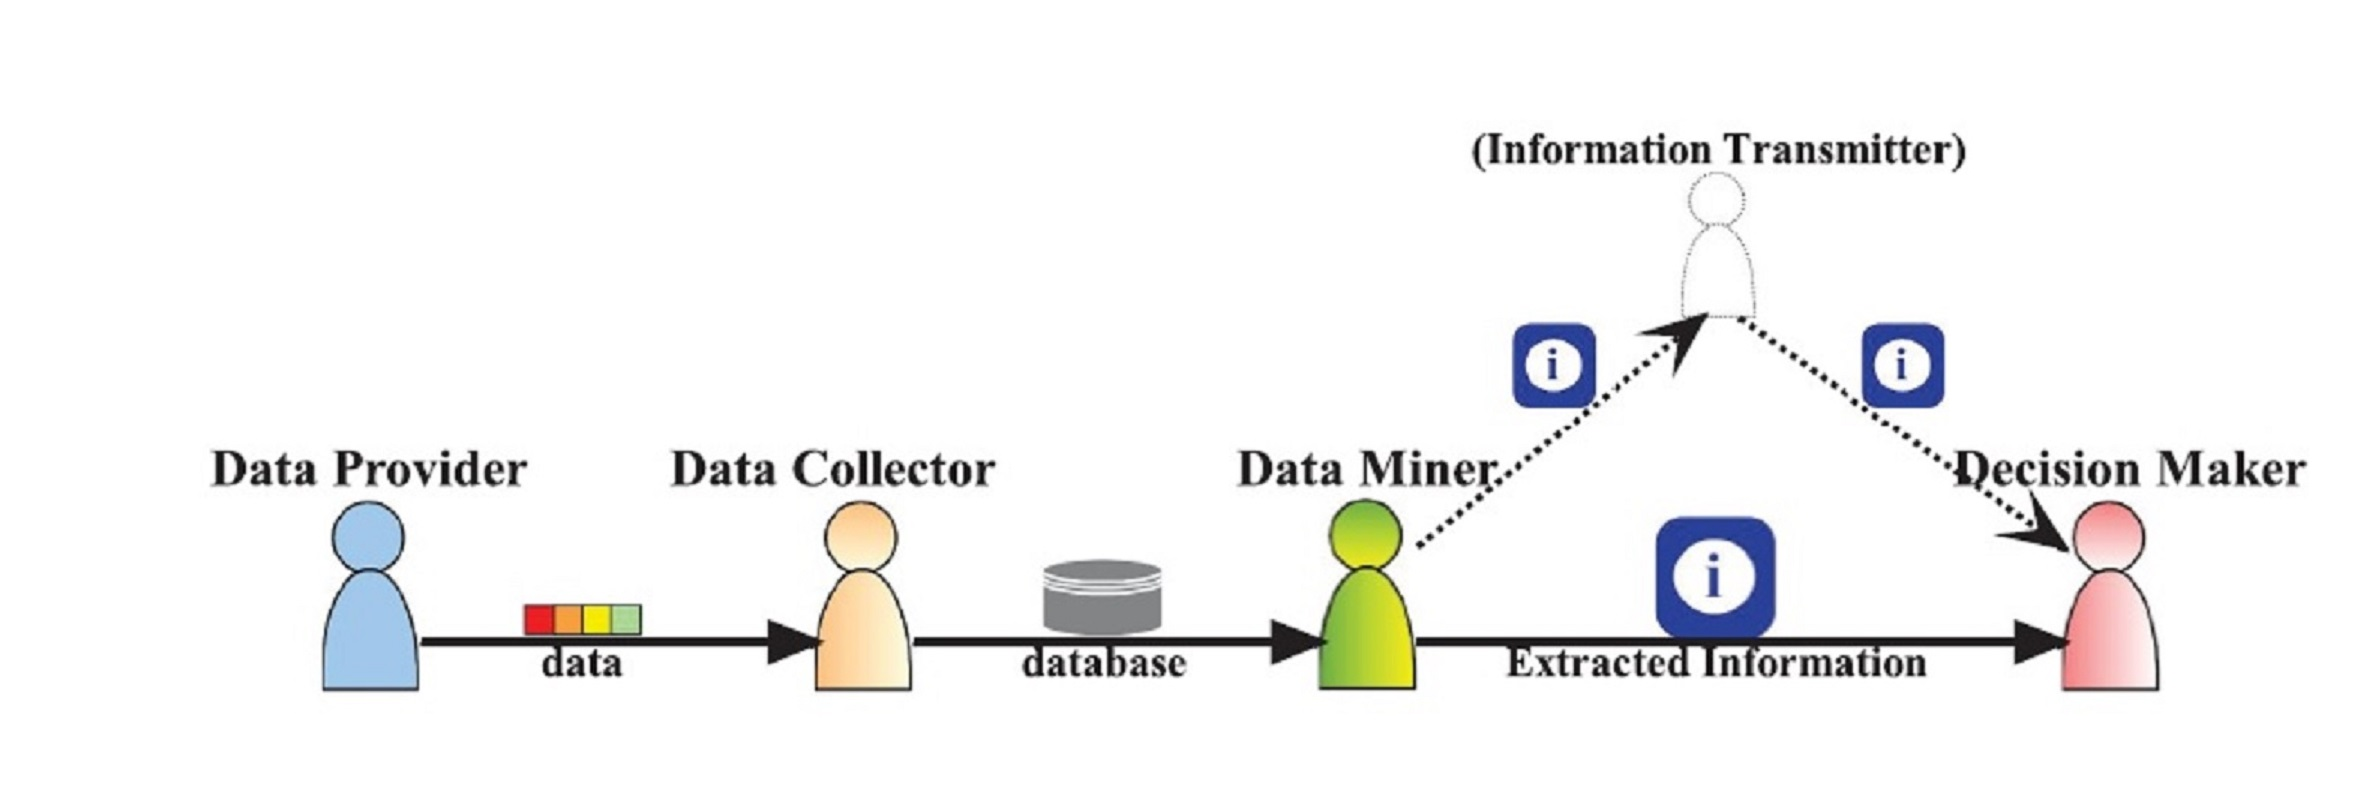
\includegraphics[width=\textwidth]{roles.jpg}
  \caption{Data Mining Roles}
\label{f:DataMiningRoles}
\end{figure*}

\begin{itemize}
 \item \textbf{Data Provider}: This would be considered a consumer who may be sharing their information online with a company during a transaction. Here, concerns around control can affect behavior \cite{Xu2014}
 \item \textbf{Data Collector}: Those who collect the users' information want to ensure that the value of the data provided is worthwhile without compromising privacy or security \cite{Xu2014}.
 \item \textbf{Data Miner}: During the process of yielding insights, this role's main concern is to keep sensitive information from unintended parties \cite{Xu2014}. 
 \item \textbf{Decision Maker}: Application, ownership, representation, and storage are privacy issues among decision makers as they seek to understand insights from the sources and people provided \cite{Xu2014}. 
 \end{itemize}

Given these concerns, there are also instances where maintaining the original data may be needed. Another approach is reversible privacy preserving data mining (RPPDM) \cite{Chen2013}. This technique still preserves data privacy but also allows for a restore procedure to take place in case there are issues that occured during the data distortion process \cite{Chen2013}. 

\subsection{Individual Access, Control, and Responsibility} 

Giving users an option to \textit{opt-in} or \textit{opt-out} of how their data is collected and used may encourage consumers to play a more active role in their online privacy. Informed consent can provide benefits and drawbacks to both companies and consumers \cite{Tene2012}. Adherence is often higher in instances where users \textit{opt-out} of certain features or functions \cite{Tene2013}. However, increased emphasis on obtaining consent can also lead to fewer innovations and benefits to society at large if consent has to be obtained for big data collection \cite{Tene2013}. Giving someone the ability to access their own information can alleviate privacy concerns but consumers are often unaware of this possibility \cite{Tene2012}.

Another option to consider is similar to that adopted by the European Union (EU), as one's \textit{right to be forgotten} where users can have their information removed from websites \cite{Francis2014}. Tools and other website information may also be available to give the users more control of their data. One tool, personal.com, allows users to gain access to personal information of theirs and control use \cite{Tene2013}. Unless individuals have a vested interest in their own privacy management, then little improvement can be expected \cite{Tene2012}. 

\subsection{Increased Onus on Companies and Organizations} 

While laws and regulations can only do so much, increased pressure by government and consumers may in fact help to entice these companies and organizations to improve their own policies and procedures in a more proactive manner \cite{Culnan2009}. Ultimately, these changes have to come from a leadership level to be effective across the organization. While one could argue doing so is part of doing \textit{good business}, these additional measures can increase costs for organizations \cite{Culnan2009}. Areas to consider could include cross-functional privacy sub-committees, privacy impact assessments (PIA), and cyber liability insurance \cite{Culnan2009}. 

\subsection{SenseMaking (Privacy by Design System)} 

With disparate data sources being prevalent in any organization, sensemaking allows for observations to live together \cite{Cavoukian2012}. This analytical big data platform was designed with privacy in mind from the ground up with key features that cannot be disabled \cite{Cavoukian2012}. Features outlined by the system include elements related to full attribution, data tethering, anonymized data analytics, audit logs that are resistant to tampering, methods that favor false negatives and correct for false positives, in addition to transfer accounting of information \cite{Cavoukian2012}. 


\section{Conclusion}
As technological capabilities, level of knowledge, personal accountability, and experience evolve, so may the level of security and process that maintains and protects one's personal identifiable information (PII). However, the possibility of data being compromised may always exist. While a consumer can take measures on their own to better protect their privacy, companies and organizations have to also be a partner in the data privacy preserving methods if they wish to use big data mining and analytics methods to their advantage. This effort also helps to keep costs down as data breaches can be very costly not only to an organization's infrastructure and resources but also to one's reputation in their effort to conduct \text{good business} with their constituents. There is no one method in particular to show how to achieve the appropriate balance of big data mining and privacy but continued effort in learning from big data breaches will help to ensure that they occur less often and with less harm to others when they do occur. 


\begin{acks}

  The author would like to thank Dr. Gregor von Laszewski and the teaching assistants for their support and guidance in writing this paper.

\end{acks}

\bibliographystyle{ACM-Reference-Format}
\bibliography{report} 


\end{document}
